\chapter{Energie, Krümmung und Strahlung}

\lectureoverview{Das Newtonsche Modell wird wesentlich aufschlussreicher, wenn man zwei Einschränkungen aufhebt. Erstens muss die Gesamtenergie einer mitbewegten Galaxie nicht genau null sein; lässt man ihre Energie beliebig, erhält man den Term \(a^{-2}\), den die allgemeine Relativitätstheorie später als räumliche Krümmung deuten wird. Zweitens muss die kosmische Quelle nicht aus druckloser Materie bestehen. Die Wellenlängen der Photonen dehnen sich mit dem Skalenfaktor, sodass sich Strahlung wie \(a^{-4}\) verdünnt und das Gesetz \(a(t)\propto t^{1/2}\) bestimmt. Ein Universum, das Materie und Strahlung enthält, wird daher bei kleinen \(a\) von Strahlung und bei größeren \(a\) von Materie dominiert. Dabei werden wir lokale Newtonsche Bewegung von globaler relativistischer Geometrie unterscheiden und die Fragen herausarbeiten, die sich ohne allgemeine Relativitätstheorie nicht beantworten lassen.}

\section{Was Newton erkennen kann}

Bevor wir das Modell erweitern, sollten wir fragen, warum die bisherige Newtonsche Rechnung überhaupt funktioniert hat. Das physikalische Universum wird durch die allgemeine Relativitätstheorie beschrieben, und seine räumliche Geometrie muss global nicht euklidisch sein. Dennoch ist jeder glatte gekrümmte Raum in einer hinreichend kleinen Umgebung näherungsweise flach. Ein kleiner Ausschnitt der Erdoberfläche erscheint eben; ebenso kann man einen Bereich des Universums, der viel kleiner als sein Krümmungsradius ist, als flach behandeln.

``Klein'' ist hier relativ zur Krümmungsskala gemeint. Der Ausschnitt kann sich trotzdem über Milliarden Lichtjahre erstrecken. Darin lassen sich benachbarte Galaxien mit Newtonscher Mechanik behandeln, sofern ihre Relativgeschwindigkeiten nichtrelativistisch und das Gravitationsfeld schwach sind. Die Newtonsche Rechnung ist also keine Konkurrenz zu Einsteins Theorie. Sie ist der lokale Grenzfall für langsame Bewegungen in der umfassenderen Beschreibung.

Hier ist sofort ein Vorbehalt angebracht. Strahlung bewegt sich nicht langsam. Photonen und Neutrinos, solange sie relativistisch sind, lassen sich nicht als Gas gewöhnlicher Newtonscher Teilchen behandeln. Die Newtonsche Überlegung wird weiterhin die Expansionsgleichung strukturieren, doch auf ihrer rechten Seite muss als Quelle an die Stelle der Ruhemassendichte die Energiedichte treten. Hier zeigt die Näherung, wo ihre Gültigkeitsgrenze liegt.

\section{Rückblick auf den Skalenfaktor}

Betrachten wir eine homogene Galaxienverteilung und ordnen wir ihr Koordinaten auf einem Gitter zu, das sich mit der mittleren kosmischen Strömung bewegt. Eine Galaxie mit fester mitbewegter Koordinate \(x\) hat vom gewählten Ursprung den physikalischen Abstand
\begin{equation}
D(t)=a(t)x
\label{eq:c02-distance}
\end{equation}
Der Skalenfaktor \(a(t)\) überführt Koordinatenabstände in physikalische Abstände.

Der Absolutwert von \(a\) ist Konvention. Skaliert man alle mitbewegten Koordinaten mit einer Konstanten um, lassen sich dieselben physikalischen Abstände durch die inverse Skalierung von \(a\) darstellen. Daher sind weder \(a\) noch die einer Koordinatenzelle zugeordnete Masse für sich genommen invariant. Verhältnisse von Skalenfaktoren und die relative Expansionsrate sind invariant:
\begin{equation}
\frac{a(t_2)}{a(t_1)},
\qquad
H(t)\equiv\frac{\dot a}{a}.
\label{eq:c02-hubble}
\end{equation}
Ist nämlich \(a'=\alpha a\) für eine feste Konstante \(\alpha\), so gilt \(\dot a'/a'=\dot a/a\).

Sei \(\nu_m\) die Masse in einem Einheitsvolumen der mitbewegten Koordinaten. Ihr Zahlenwert ändert sich, wenn man das Gitter umbenennt; bei Erhaltung gewöhnlicher Materie bleibt er jedoch zeitlich konstant. Ein mitbewegter Einheitswürfel hat das physikalische Volumen \(a^3\), also ist die Materiedichte
\begin{equation}
\boxed{\rho_m(a)=\frac{\nu_m}{a^3}.}
\label{eq:c02-matter-density}
\end{equation}
Diese Verdünnung wie \(a^{-3}\) ergibt sich schlicht aus der Volumenzunahme: Die Ruheenergie im mitbewegten Kasten bleibt gleich, während sein Volumen wächst.

Reale Galaxien sind nicht starr am Gitter befestigt. Sie umkreisen einander in Gruppen, fallen in Galaxienhaufen und besitzen kleine Geschwindigkeiten relativ zur mittleren Strömung. Der Skalenfaktor beschreibt die geglättete Bewegung auf großen Skalen; solche lokalen Abweichungen nennt man \emph{Pekuliargeschwindigkeiten}.

\begin{classroomqa}
\audiencequestion{Muss sich jede Galaxie genau radial von jeder anderen Galaxie entfernen?}
\lecturerresponse{Nur die gemittelte Hubble-Strömung hat diese Form. Die tatsächliche Bewegung einer Galaxie setzt sich aus der gemeinsamen Expansion und einer durch nahe Strukturen verursachten Pekuliargeschwindigkeit zusammen. Der Unterschied ist wie bei einer Flussströmung mit überlagerten Wirbeln: Die Wirbel sind lokal bedeutsam, ohne die großräumige Strömung aufzuheben. \lecturetimestamp{00:24:47--00:26:33}}
\end{classroomqa}

Für drucklose Materie mit Newtonscher Gesamtenergie null ergab die vorherige Vorlesung
\begin{equation}
H^2=\frac{8\pi G}{3}\rho_m
=\frac{8\pi G\nu_m}{3a^3}.
\label{eq:c02-zero-energy-friedmann}
\end{equation}
Da die Gesamtnormierung des Gitters beliebig ist, können wir vorübergehend Einheiten wählen, für die \(8\pi G\nu_m/3=1\) gilt. Auf dem expandierenden Zweig gilt
\begin{equation}
\frac{\dot a}{a}=\frac{1}{a^{3/2}},
\qquad
\dot a=\frac{1}{\sqrt a}.
\end{equation}
Löst man nach der Ableitung auf und integriert, erhält man
\begin{equation}
\frac{dt}{da}=\sqrt a,
\qquad
t-t_B=\frac{2}{3}a^{3/2},
\end{equation}
wobei \(t_B\) der Zeitpunkt ist, zu dem diese idealisierte Lösung \(a=0\) erreicht. Somit gilt
\begin{equation}
\boxed{a(t)\propto (t-t_B)^{2/3}.}
\label{eq:c02-matter-law}
\end{equation}
In diesem kritischen Modell, das nur Materie enthält, expandiert das Universum für immer. Seine Expansion verlangsamt sich, weil \(\dot a\propto a^{-1/2}\) gilt, aber \(\dot a\) wird für keinen endlichen Wert von \(a\) null.

\begin{figure}[ht]
\centering
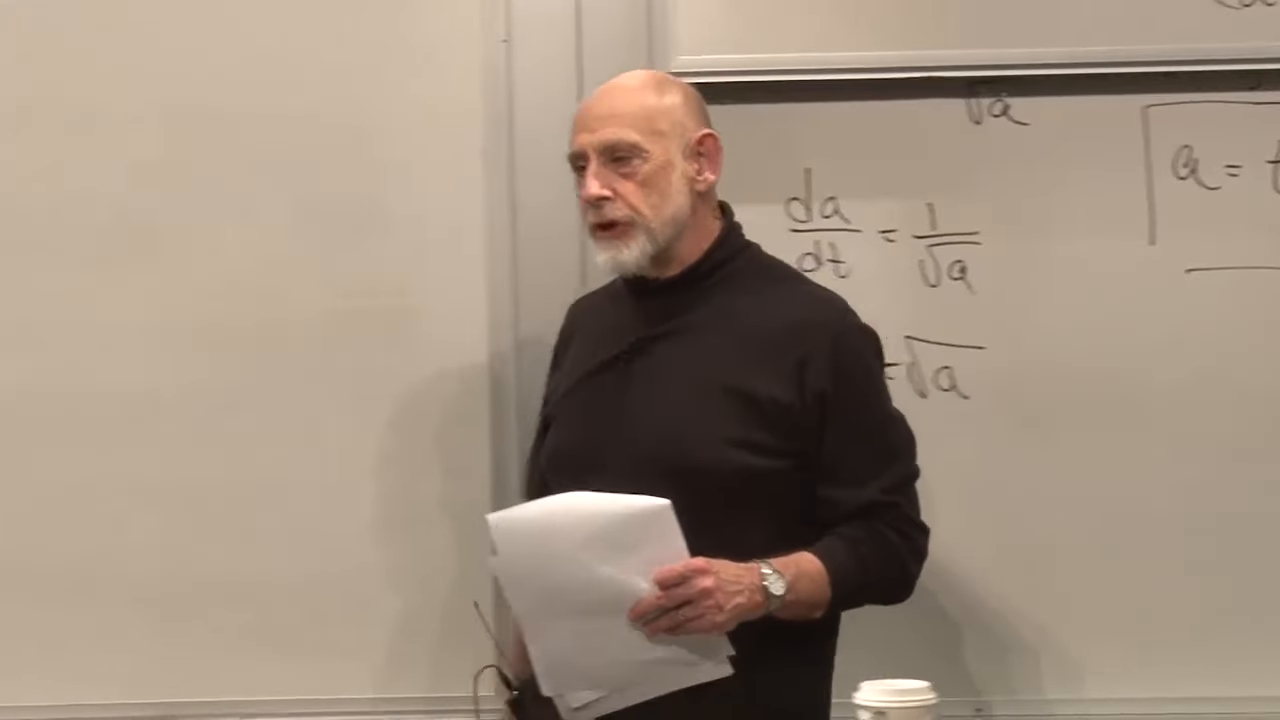
\includegraphics[width=0.68\textwidth]{lecture_02_figure_02.png}
\caption{Die Wiederholungstafel hält \(\dot a=1/\sqrt a\) sowie das eingerahmte Gesetz für materiedominierte Expansion \(a\propto t^{2/3}\) fest. Die Zwischenschritte der Algebra sind teilweise verdeckt und werden durch die Gleichungen ~\eqref{eq:c02-zero-energy-friedmann}--\eqref{eq:c02-matter-law} ergänzt.}
\label{fig:c02-matter-recap}
\lectureframe{00:29:20.838}
\end{figure}

\begin{classroomqa}
\audiencequestion{Warum wurde die negative Quadratwurzel verworfen?}
\lecturerresponse{Sie wurde von der Gleichung nicht verworfen. Gleichung~\eqref{eq:c02-zero-energy-friedmann} legt \(H^2\) fest, nicht aber das Vorzeichen von \(H\). Die positive Wurzel beschreibt Expansion, die negative Kontraktion. Ein Stein im Gravitationsfeld eines Planeten kann sich nach außen oder nach innen bewegen und dabei dieselbe Energiegleichung erfüllen; die Anfangsbedingung wählt den Zweig. Wir haben den expandierenden Zweig gewählt, weil es um das Universum geht, in dem wir leben. \lecturetimestamp{00:23:09--00:24:46}}
\end{classroomqa}

Im nächsten Modell lassen wir die Dunkle Energie weiterhin weg. Das ist beabsichtigt: Zunächst wollen wir das ältere Modell aus Materie und Strahlung verstehen, bevor wir die Komponente hinzufügen, die die heutige beschleunigte Epoche bestimmt. Dunkle Materie ist dagegen bereits im Materieterm enthalten, denn auch nichtrelativistische dunkle Materie verdünnt sich wie \(a^{-3}\).

\begin{classroomqa}
\audiencequestion{Ist die Dunkle Energie heute nicht die dominante Komponente?}
\lecturerresponse{Doch. Die hier entwickelte Geschichte mit zwei Komponenten entspricht der üblichen Lehrbuchkosmologie aus der Zeit vor der Entdeckung der heutigen beschleunigten Expansion. Dunkle Materie gehört zur Materie; Dunkle Energie ist eine dritte Komponente, die gesondert eingeführt wird. Wenn wir mit dem älteren Modell beginnen, sehen wir, was jeder zusätzliche Term verändert. \lecturetimestamp{00:28:02--00:28:45}}
\end{classroomqa}

\section{Die Energiekonstante wieder einsetzen}

Die Wahl einer Energie von null ist eine spezielle Anfangsbedingung. Um sie aufzuheben, betrachten wir wieder eine Galaxie der Masse \(m\) am Rand einer homogenen Kugel. Ihr mitbewegter Radius sei \(x\), sodass
\begin{equation}
D=ax,
\qquad
\dot D=\dot a x.
\label{eq:c02-comoving-particle}
\end{equation}
Nach dem Newtonschen Schalentheorem beeinflusst nur die Masse \(M(D)\) innerhalb der Kugel die radiale Beschleunigung; äußere Kugelschalen üben keine resultierende Kraft aus. Die erhaltene Newtonsche Energie der Galaxie ist
\begin{equation}
\frac{1}{2}m\dot D^{\,2}-\frac{GM(D)m}{D}=E.
\label{eq:c02-newton-energy}
\end{equation}
Der Faktor \(m\) gehört in beide Terme. Beim schnellen Schreiben an der Tafel lässt man ihn leicht weg; mit ihm wird jedoch deutlich, dass die endgültige Konstante die Energie pro Testmasse ist.

Wegen der Homogenität können wir die repräsentative Galaxie bei \(x=1\) wählen. Dann gilt \(D=a\) und \(\dot D=\dot a\), und die Kugel hat das Volumen
\begin{equation}
V_{\rm sph}=\frac{4\pi}{3}a^3,
\qquad
M(a)=\rho_m V_{\rm sph}=\frac{4\pi}{3}\rho_m a^3.
\label{eq:c02-enclosed-mass}
\end{equation}
An der Tafel steht \(V\) sowohl für das Volumen als auch, in einer Randnotiz, für die Radialgeschwindigkeit. Wir verwenden stattdessen die eindeutigen Symbole \(V_{\rm sph}\) und \(\dot D\).

\begin{figure}[ht]
\centering
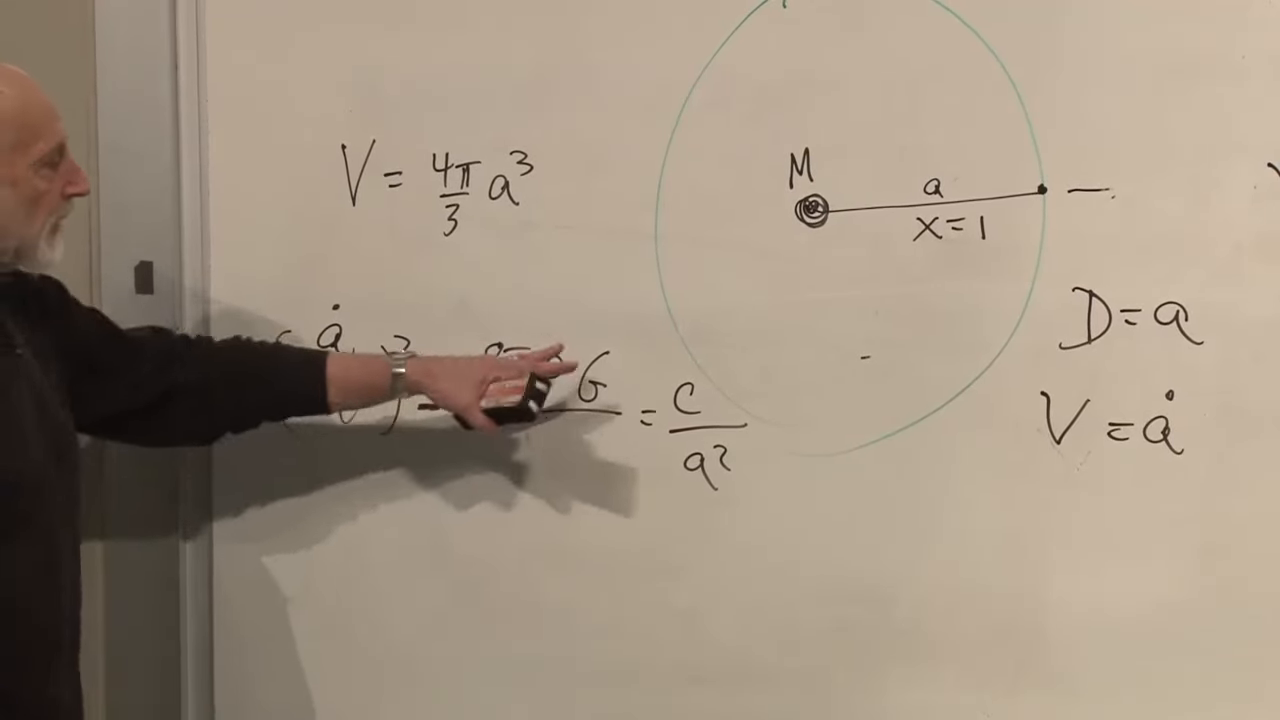
\includegraphics[width=0.86\textwidth]{lecture_02_figure_03.png}
\caption{Die Kugel mit der eingeschlossenen Masse und die Friedmann-Gleichung für von null verschiedene Energie. Zu den sichtbaren Beschriftungen gehören \(V_{\rm sph}=4\pi a^3/3\), die zentrale Masse \(M\), \(x=1\), \(D=a\) und \(\dot D=\dot a\). Ein Teil der Gleichung ist durch den Dozenten verdeckt und wird im Folgenden algebraisch rekonstruiert.}
\label{fig:c02-energy-board}
\lectureframe{00:37:59.876}
\end{figure}

\begin{figure}[ht]
\centering
\begin{tikzpicture}[scale=1.05,>=Latex]
  \draw[thick] (0,0) circle (2.6);
  \fill (0,0) circle (2.2pt) node[below left=2pt] {\(M(a)\)};
  \draw[thick,->] (0,0) -- (2.58,0);
  \fill (2.6,0) circle (2.2pt) node[right=4pt] {galaxy \(m\)};
  \node[above] at (1.30,0.04) {\(D=ax\)};
  \node[below] at (1.30,-0.04) {\(x=1\Rightarrow D=a\)};
  \draw[->,blue!60!black,thick] (2.63,0.18) -- (3.55,0.72)
    node[right] {\(\dot D=\dot a\)};
  \node at (0,-3.05) {\(M(a)=\frac{4\pi}{3}\rho_m a^3\)};
\end{tikzpicture}
\caption{Eine saubere Rekonstruktion der Newtonschen Kugel bei \(x=1\). Die äußeren Schalen heben einander auf, sodass die Galaxie am Rand nur auf die eingeschlossene Masse reagiert.}
\label{fig:c02-sphere-redraw}
\end{figure}

Setzen wir \(D=a\) in Gleichung~\eqref{eq:c02-newton-energy} ein, teilen durch \(m/2\) und definieren die Konstante
\begin{equation}
C\equiv\frac{2E}{m}.
\end{equation}
Dann erhalten wir
\begin{equation}
\dot a^{\,2}-\frac{2GM(a)}{a}=C.
\label{eq:c02-energy-a}
\end{equation}
Durch Division durch \(a^2\) und unter Verwendung von Gleichung~\eqref{eq:c02-enclosed-mass} folgt
\begin{equation}
\left(\frac{\dot a}{a}\right)^2-
\frac{8\pi G}{3}\rho_m=\frac{C}{a^2},
\label{eq:c02-energy-form}
\end{equation}
oder gleichwertig
\begin{equation}
\boxed{H^2=\frac{8\pi G}{3}\rho_m+\frac{C}{a^2}.}
\label{eq:c02-friedmann-C}
\end{equation}
Dies ist die erste Friedmann-Gleichung für drucklose Materie, formuliert in der Newtonschen Energiekonvention. Der neue Term \(a^{-2}\) hält fest, ob die repräsentative Galaxie mit einer Energie oberhalb, genau bei oder unterhalb der Fluchtenergie gestartet ist.

Setzt man \(\rho_m=\nu_m/a^3\) ein, ist es zweckmäßig, \begin{equation}
A_m\equiv\frac{8\pi G\nu_m}{3}>0,
\end{equation} zu definieren, sodass
\begin{equation}
H^2=\frac{A_m}{a^3}+\frac{C}{a^2},
\qquad
\dot a^{\,2}=\frac{A_m}{a}+C.
\label{eq:c02-energy-branches}
\end{equation}
gilt. Die Gleichung ist aufschlussreicher, wenn man sie zunächst anhand ihrer Grenzfälle betrachtet, statt sie sofort zu integrieren.

\subsection{Positive Energie}

Falls \(C>0\) gilt, dominiert bei kleinen \(a\) der Materieterm \(A_m/a^3\). Die frühe Expansion folgt daher weiterhin dem Materiegesetz \(a\propto t^{2/3}\). Bei großen \(a\) dominiert jedoch in \(H^2\) der Term \(C/a^2\), oder gleichwertig
\begin{equation}
\dot a^{\,2}\longrightarrow C.
\end{equation}
Die Expansion nähert sich einer konstanten Geschwindigkeit an:
\begin{equation}
a(t)\sim\sqrt C\,t.
\label{eq:c02-positive-late}
\end{equation}
Das ist das kosmologische Gegenstück dazu, einen Apfel schneller als mit Fluchtgeschwindigkeit zu werfen. Die Gravitation verringert seine Geschwindigkeit fortwährend, doch weit entfernt behält der Apfel eine von null verschiedene asymptotische Geschwindigkeit.

\subsection{Null Energie}

Für \(C=0\) liefert Gleichung~\eqref{eq:c02-energy-branches} wieder die kritische Lösung \(a\propto t^{2/3}\). Die Expansion setzt sich unbegrenzt fort, während \(\dot a\) gegen null geht. Dies ist genau der Fall mit Fluchtenergie.

\subsection{Negative Energie}

Falls \(C=-|C|<0\) gilt, dann
\begin{equation}
H^2=\frac{A_m}{a^3}-\frac{|C|}{a^2}
=\frac{A_m-|C|a}{a^3}.
\label{eq:c02-negative-energy}
\end{equation}
Der Skalenfaktor kann nicht größer werden als
\begin{equation}
a_{\max}=\frac{A_m}{|C|},
\label{eq:c02-amax}
\end{equation}
denn dort wird die rechte Seite null. Der expandierende Zweig erreicht \(a_{\max}\) mit \(\dot a=0\); danach setzt sich die Lösung auf dem kontrahierenden Zweig fort. Im Newtonschen Bild entspricht dies einem Apfel, der mit weniger als der Fluchtgeschwindigkeit gestartet wird: Er steigt, kehrt um und fällt zurück.

\begin{classroomqa}
\audiencequestion{Wie kann das Modell rekollabieren, wenn die rechte Seite \(H^2\) beträgt und daher nicht negativ sein kann?}
\lecturerresponse{Sie wird niemals negativ. Während der Expansion nimmt die rechte Seite bis auf null bei \(a_{\max}\) ab. Dort gilt \(H=0\). Anschließend wechselt die Lösung von der positiven zur negativen Quadratwurzel und durchläuft den erlaubten Bereich mit \(\dot a<0\) in umgekehrter Richtung. Eine verlockende, aber falsche Fortsetzung ließe den Ausdruck durch null hindurchgehen. Das ist nicht möglich: Null ist die Grenze und kein Wert, durch den ein reelles \(H\) fortgesetzt werden kann. \lecturetimestamp{00:48:43--00:53:03}}
\end{classroomqa}

Damit ergeben die drei Newtonschen Energien drei qualitativ verschiedene Verläufe: Rekollaps für \(C<0\), kritisches Entweichen für \(C=0\) und ewige Expansion mit asymptotisch konstanter \(\dot a\) für \(C>0\). Der überraschende nächste Schritt ist, dass die allgemeine Relativitätstheorie denselben Fällen eine geometrische Bedeutung zuordnet.

\enlargethispage{1pt}
\section{Von der Energie zur Krümmung}

Bringen wir den Energieterm in Gleichung~\eqref{eq:c02-friedmann-C} auf die geometrische Seite und definieren
\begin{equation}
k\equiv-C.
\label{eq:c02-k-definition}
\end{equation}
Dann gilt
\begin{equation}
\boxed{H^2+\frac{k}{a^2}=\frac{8\pi G}{3}\rho.}
\label{eq:c02-friedmann-k}
\end{equation}
An der Tafel wechseln die Symbole zwischen \(C\), \(K\) und \(\kappa\); beim Verschieben des Terms über das Gleichheitszeichen wird ein Vorzeichen in die Definition aufgenommen. Gleichung~\eqref{eq:c02-k-definition} legt unsere Konvention fest: Positive Newtonsche Energie entspricht \(k<0\), Energie null entspricht \(k=0\) und negative Newtonsche Energie entspricht \(k>0\).

\begin{figure}[ht]
\centering
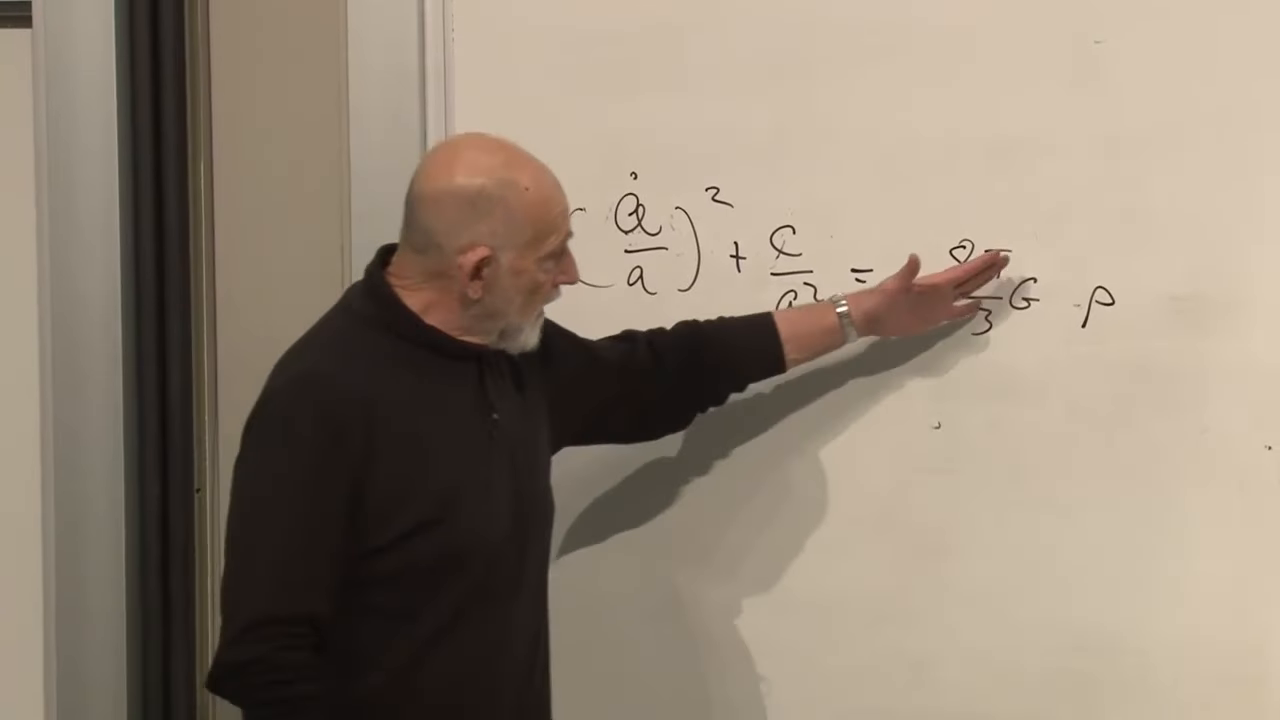
\includegraphics[width=0.76\textwidth]{lecture_02_figure_04.png}
\caption{Die Friedmann-Gleichung, angeordnet mit der Geometrie links und der Quelle rechts. Die Abbildung veranschaulicht diese begriffliche Aufteilung; sie zeigt nicht die vollständige Einsteinsche Feldgleichung.}
\label{fig:c02-geometry-source}
\lectureframe{00:55:22.810}
\end{figure}

Diese Anordnung ist eine Miniaturversion von Einsteins Gleichung. Die linke Seite beschreibt die Geometrie: die Expansion durch \(H\) und die räumliche Krümmung durch \(k/a^2\). Die rechte Seite beschreibt die materielle Quelle. In der Newtonschen Mechanik war diese Quelle die Massendichte. In der Relativitätstheorie besteht sie aus Energie und Impuls, vollständig dargestellt durch den Energie-Impuls-Tensor. Für ein homogenes und isotropes Universum hängt die erste Friedmann-Gleichung von der gesamten Energiedichte \(\rho\) ab.

Behält man die gewöhnlichen Einheiten bei, trägt eine Massendichte über ihre Ruheenergie \(\rho_{\rm mass}c^2\) bei. Von hier an setzen wir \(c=1\), sodass Masse und Energie in denselben Einheiten angegeben werden. Das Symbol \(\rho\) kann dann Ruhemasse, kinetische Energie, Strahlung und jede andere homogene Energiekomponente umfassen.

\begin{figure}[ht]
\centering
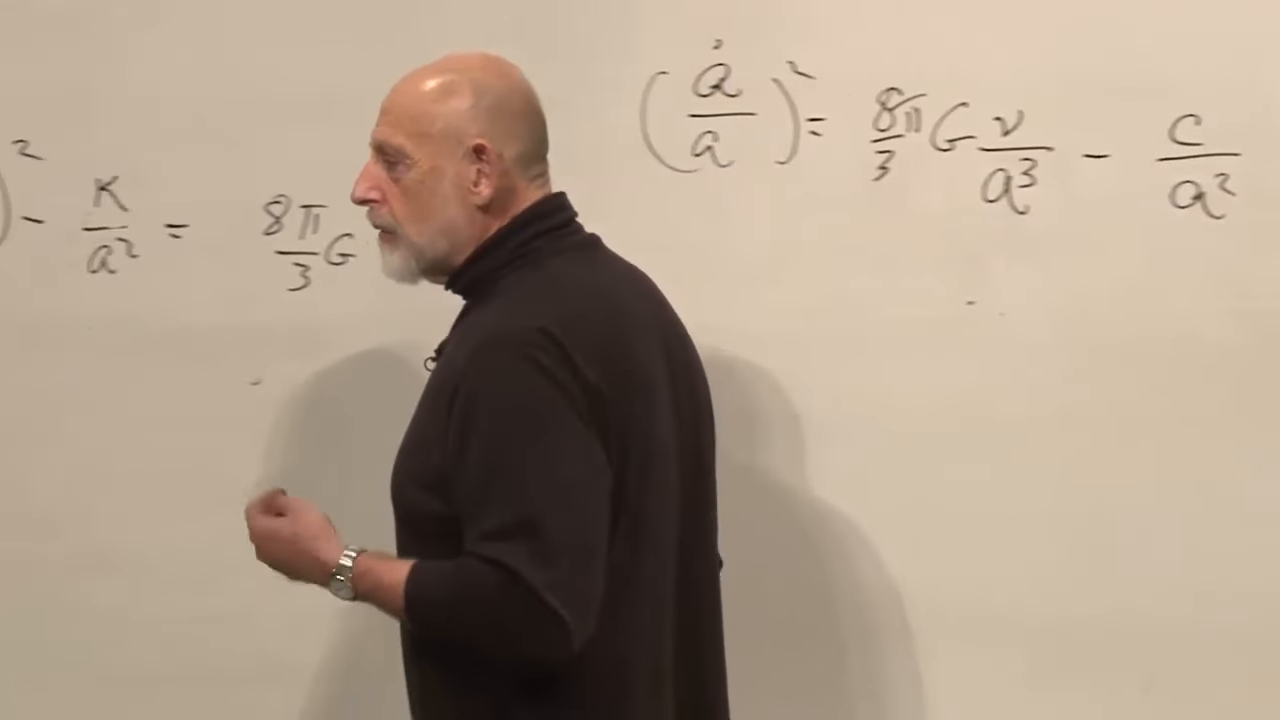
\includegraphics[width=0.88\textwidth]{lecture_02_figure_05.png}
\caption{Gegenüberstellungen der Friedmann-Gleichung an der Tafel: eine Krümmungsform mit \(\rho\) und eine Materieform, die sich nach Einsetzen von \(\rho_m=\nu_m/a^3\) ergibt. Die Schreibweise an der Tafel wechselt; Gleichung~\eqref{eq:c02-k-definition} hält die hier verwendete Vorzeichenkonvention fest.}
\label{fig:c02-curvature-comparison}
\lectureframe{00:57:52.659}
\end{figure}

Die geometrische Deutung ist global. Im relativistischen Modell beschreibt \(k=0\) flache räumliche Schnitte, \(k>0\) positiv gekrümmte sphärische Schnitte und \(k<0\) negativ gekrümmte hyperbolische Schnitte. Die Newtonsche Herleitung ergab dieselbe Entwicklungsgleichung, ohne über diese globalen Geometrien zu verfügen. Ihre von null verschiedene Energiekonstante ist also eine bemerkenswert genaue Nachbildung der Krümmung, aber keine Herleitung des gekrümmten Raums selbst.

\begin{classroomqa}
\audiencequestion{Wie können die Newtonsche Mechanik und die allgemeine Relativitätstheorie dieselbe Expansionsgleichung ergeben, wenn ihre Geometrien verschieden sind?}
\lecturerresponse{Die allgemeine Relativitätstheorie schließt den flachen Fall ein, und jede glatte Geometrie ist lokal näherungsweise flach. Noch bemerkenswerter ist, dass die Newtonsche Energiekonstante in der Entwicklungsgleichung genau an der Stelle auftritt, die in der Relativitätstheorie von der räumlichen Krümmung eingenommen wird. Die dynamische Formel stimmt überein, die globale Deutung jedoch nicht: Der euklidische Newtonsche Raum ist nicht heimlich zu einer Kugel oder einem hyperbolischen Raum geworden. Diese drei Geometrien müssen innerhalb der allgemeinen Relativitätstheorie konstruiert werden. \lecturetimestamp{01:20:59--01:24:20}}
\end{classroomqa}

\section{Strahlung in einem expandierenden Kasten}

Nun ändern wir den Inhalt des Universums. Betrachten wir einen mitbewegten Einheitswürfel. Sein physikalisches Volumen ist \(a^3\). Für nichtrelativistische Materie ist die Teilchenzahl in diesem Kasten fest, und die Ruheenergie jedes Teilchens bleibt näherungsweise konstant; daraus folgt \(\rho_m\propto a^{-3}\). Bei Strahlung kommt ein weiterer Effekt hinzu: Jedes Photon verliert Energie, während sich das Universum ausdehnt.

Ein Photon mit der Wellenlänge \(\lambda\) hat die Energie
\begin{equation}
E_\gamma=\frac{hc}{\lambda},
\qquad
E_\gamma\propto\lambda^{-1}.
\label{eq:c02-photon-energy}
\end{equation}
Bei homogener Expansion dehnt sich die Wellenlänge einer frei laufenden Welle mit dem Skalenfaktor:
\begin{equation}
\frac{\lambda(t_2)}{\lambda(t_1)}
=\frac{a(t_2)}{a(t_1)},
\qquad
\lambda\propto a.
\label{eq:c02-redshift}
\end{equation}
Das ist die kosmologische Rotverschiebung. Daraus folgt
\begin{equation}
E_\gamma\propto a^{-1}.
\label{eq:c02-photon-redshift}
\end{equation}
Wenn die Photonenzahl im mitbewegten Kasten erhalten bleibt, nimmt seine gesamte Strahlungsenergie wie \(a^{-1}\) ab. Teilt man durch sein physikalisches Volumen \(a^3\), erhält man
\begin{equation}
\boxed{\rho_r(a)=\frac{\nu_r}{a^4}.}
\label{eq:c02-radiation-density}
\end{equation}
Dabei ist \(\nu_r\) die konstante Amplitude der Dichte frei strömender Strahlung. Bei Strahlung kommt eine zusätzliche inverse Potenz von \(a\) hinzu: drei Potenzen durch die räumliche Verdünnung und eine durch die Rotverschiebung jedes Photons.

Die Analogie mit einer Gitarrensaite vermittelt eine hilfreiche Anschauung. Eine auf die Saite passende Mode hat eine ganzzahlige Anzahl von halben Wellenlängen. Wird die Saite langsam verlängert, kann sich diese Zahl nicht kontinuierlich ändern; stattdessen passt sich die Wellenlänge an die neue Länge an. Ebenso ist bei einer Welle auf einem langsam expandierenden Ring die Knotenzahl eine adiabatische Invariante, sodass ihre Wellenlänge dem Umfang folgt. Eine allgemeine Welle lässt sich in solche Moden zerlegen.

Das ersetzt keine Lösung der Maxwell-Gleichungen in einer expandierenden Raumzeit. Es liefert die kontrollierte Anschauung hinter Gleichung~\eqref{eq:c02-redshift}: Die langsame geometrische Expansion ändert die physikalische Wellenlänge, während die Modenkennzeichnung erhalten bleibt.

\begin{classroomqa}
\audiencequestion{Erfordert dieses Argument einen leitenden oder reflektierenden Kasten? Was geschieht im leeren expandierenden Raum ohne physische Wände?}
\lecturerresponse{Die Wände dienen der Buchführung; damit ist nicht gemeint, dass das Universum von einem Leiter umschlossen wäre. Ein vollständiger Beweis ergibt sich aus der Wellenausbreitung in der expandierenden Metrik. Für die vorliegende Überlegung verwenden wir die beobachtete und relativistisch hergeleitete Tatsache, dass sich frei laufende Wellenlängen proportional zu \(a\) ändern. Der Kasten hilft, die Photonen und das physikalische Volumen zu zählen; er verursacht nicht die kosmologische Rotverschiebung. \lecturetimestamp{01:02:21--01:04:37}}
\end{classroomqa}

\begin{classroomqa}
\audiencequestion{Warum sollte sich eine Wellenlänge am Gitter orientieren, statt eine feste physikalische Länge beizubehalten?}
\lecturerresponse{Betrachten wir eine Mode auf einem Ring, dessen Umfang sich adiabatisch ändert. Ihre ganzzahlige Knotenzahl kann nicht kontinuierlich variieren, also muss sich die zulässige Wellenlänge mit dem Ring ändern. Zerlegt man eine allgemeine Welle in Fourier-Moden, ergibt sich dieselbe Schlussfolgerung für jede Mode einzeln. Das liefert die nötige adiabatische Anschauung; die exakte Aussage gehört zur Feldtheorie in gekrümmter Raumzeit. \lecturetimestamp{01:34:18--01:38:33}}
\end{classroomqa}

\subsection{Die strahlungsdominierte Lösung}

Lassen wir die Krümmung zunächst weg und setzen Gleichung~\eqref{eq:c02-radiation-density} in die Friedmann-Gleichung ein:
\begin{equation}
H^2=\frac{8\pi G\nu_r}{3a^4}
\equiv\frac{A_r}{a^4},
\qquad A_r>0.
\label{eq:c02-radiation-friedmann}
\end{equation}
Auf dem expandierenden Zweig gilt
\begin{equation}
\frac{\dot a}{a}=\frac{\sqrt{A_r}}{a^2},
\qquad
\dot a=\frac{\sqrt{A_r}}{a}.
\end{equation}
Daher
\begin{equation}
a\,da=\sqrt{A_r}\,dt,
\qquad
\frac{a^2}{2}=\sqrt{A_r}(t-t_B),
\end{equation}
und
\begin{equation}
\boxed{a(t)\propto(t-t_B)^{1/2}.}
\label{eq:c02-radiation-law}
\end{equation}
Der Unterschied zwischen den Exponenten \(1/2\) und \(2/3\) mag optisch gering erscheinen, ist physikalisch aber entscheidend. Expansionsrate, Temperatur, das Einfrieren von Reaktionen und die Horizontgröße im frühen Universum hängen davon ab, welche Komponente dominiert.

\section{Ein Universum aus Materie und Strahlung}

Für getrennt erhaltene Materie und Strahlung addieren sich ihre Dichten:
\begin{equation}
\rho(a)=\rho_m(a)+\rho_r(a).
\end{equation}
Lässt man die Krümmung für diesen Vergleich außer Acht, gilt
\begin{equation}
\boxed{H^2=\frac{C_m}{a^3}+\frac{C_r}{a^4},}
\label{eq:c02-mixed-friedmann}
\end{equation}
wobei \(C_m,C_r>0\). An der Tafel werden die beiden Koeffizienten zunächst mit \(C_1\) und \(C\) bezeichnet; mündlich wird das zweite Symbol zu einer eigenen Konstanten berichtigt. Die Schreibweise in Gleichung~\eqref{eq:c02-mixed-friedmann} macht diese Korrektur ausdrücklich kenntlich.

\begin{figure}[ht]
\centering
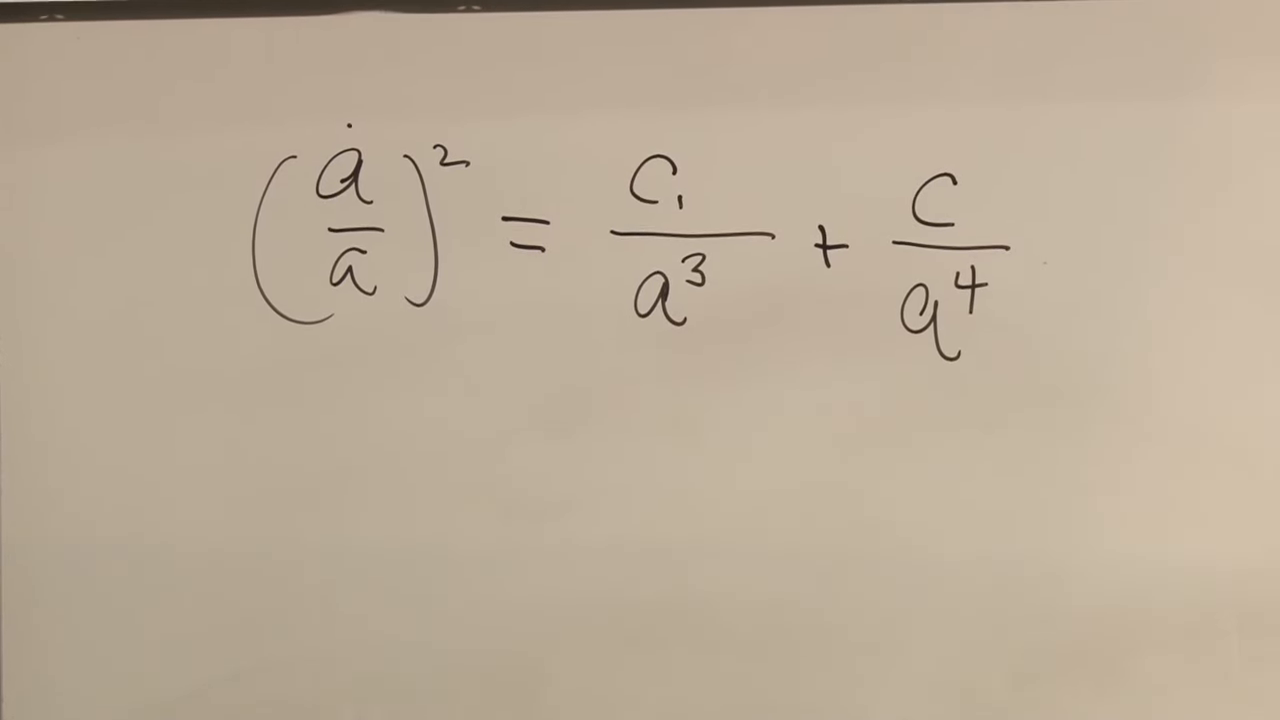
\includegraphics[width=0.74\textwidth]{lecture_02_figure_06.png}
\caption{Die gemischte Materie-Strahlungs-Gleichung an der Tafel. Der schriftlich notierte zweite Koeffizient wird anschließend zu einer strahlungsspezifischen Konstante berichtigt, die in Gleichung~\eqref{eq:c02-mixed-friedmann} mit \(C_r\) bezeichnet ist.}
\label{fig:c02-mixed-board}
\lectureframe{01:11:37.997}
\end{figure}

Bei kleinen \(a\) überwiegt der Strahlungsterm, weil \(a^{-4}\) schneller wächst als \(a^{-3}\):
\begin{equation}
a\ll a_{\rm eq}
\quad\Longrightarrow\quad
H^2\simeq\frac{C_r}{a^4},
\qquad
a(t)\propto t^{1/2}.
\end{equation}
Bei größeren \(a\) überwiegt die Materie:
\begin{equation}
a\gg a_{\rm eq}
\quad\Longrightarrow\quad
H^2\simeq\frac{C_m}{a^3},
\qquad
a(t)\propto t^{2/3}.
\end{equation}
Die Gleichheitsskala ergibt sich unmittelbar, indem man die beiden Terme gleichsetzt:
\begin{equation}
a_{\rm eq}=\frac{C_r}{C_m}.
\label{eq:c02-equality-scale}
\end{equation}
Dieser Gleichheitszeitpunkt ist nicht dasselbe Ereignis wie die Entkopplung der Photonen. Bei der Gleichheit geht es darum, wann die beiden Energiedichten übereinstimmen; bei der Entkopplung darum, wann Wechselwirkungen Materie und Strahlung nicht länger im thermischen Kontakt halten.

Zum Strahlungssektor gehören Photonen und alle Teilchenarten, die sich ultrarelativistisch bewegen. Sehr leichte Neutrinos verhalten sich bei hinreichend hohen Temperaturen so; ein Hintergrund aus Gravitonen würde sich ebenso entwickeln. Wird eine massive Teilchenart nichtrelativistisch, beginnt ihr dominanter Ruhemassebeitrag wie Materie zu skalieren. Kalte dunkle Materie gehört zu \(C_m/a^3\) und nicht zum Strahlungsterm.

\begin{classroomqa}
\classquestion{Welcher Term in Gleichung~\eqref{eq:c02-mixed-friedmann} dominiert zuerst und welcher später?}
\lecturerresponse{Bei kleinen \(a\) wächst \(a^{-4}\) schneller als \(a^{-3}\); daher bestimmt Strahlung die frühe Expansion und es gilt \(a\propto t^{1/2}\). Mit zunehmendem \(a\) fällt das Verhältnis von Strahlung zu Materie wie \(1/a\); dann bestimmt Materie die Expansion und es gilt \(a\propto t^{2/3}\). \lecturetimestamp{01:11:46--01:13:38}}
\end{classroomqa}

\begin{classroomqa}
\audiencequestion{Wird angenommen, dass die relativen Anteile von Materie und Strahlung konstant sind?}
\lecturerresponse{Ihre Dichten sind nicht konstant, aber die Koeffizienten \(C_m\) und \(C_r\) können als konstant behandelt werden, sobald die Komponenten keine Energie mehr effizient austauschen und Teilchenentstehung oder -vernichtung vernachlässigbar ist. Dann bleibt die mitbewegte Ruhemasse der Materie erhalten, ebenso wie die mitbewegte Photonenzahl frei laufender Strahlung; die Rotverschiebung liefert den zusätzlichen Faktor \(a^{-1}\). In Epochen starker Wechselwirkung oder bei der Annihilation von Teilchenarten muss die Buchführung verfeinert werden. \lecturetimestamp{01:13:39--01:14:53}}
\end{classroomqa}

\begin{classroomqa}
\audiencequestion{Wann hörten Materie und Strahlung auf, stark miteinander zu wechselwirken?}
\lecturerresponse{Eine grobe Größenordnung für die Entkopplung der Photonen von gewöhnlicher Materie ist \(10^5\) Jahre. Die genaue Rekombinationsgeschichte wird später berechnet und darf nicht mit dem Materie--Strahlungs-Gleichheitszeitpunkt verwechselt werden. Hier kommt es nur darauf an, dass sich die beiden Komponenten nach der Entkopplung näherungsweise getrennt verfolgen lassen. \lecturetimestamp{01:27:29--01:27:46}}
\end{classroomqa}

\begin{classroomqa}
\audiencequestion{Woher wissen wir, dass es eine frühe Epoche mit \(a\propto t^{1/2}\) gab, bevor Galaxien die Expansion nachzeichnen konnten?}
\lecturerresponse{Wir erschließen die Expansionsgeschichte aus den physikalischen Spuren, die sie hinterlassen hat. Die primordiale Nukleosynthese hängt vom frühen Wettstreit zwischen Reaktionsraten und \(H(t)\) ab; die kosmische Mikrowellenhintergrundstrahlung zeichnet den späteren thermischen Zustand und die Störungen auf. Beobachtungen von Galaxien machen das Verhalten während der Materieepoche unmittelbarer sichtbar, während die Strahlungsepoche anhand dieser Belege aus dem frühen Universum rekonstruiert wird. \lecturetimestamp{01:27:46--01:30:10}}
\end{classroomqa}

Das Modell aus Materie und Strahlung ist bewusst unvollständig. Es ist der klassische Rahmen, in dem das Universum von Strahlungs- zu Materiedominanz übergeht. Die heutige beschleunigte Expansion erfordert eine weitere Quelle, die Dunkle Energie; sie fügt einen qualitativ anderen Term hinzu.

\section{Wohin die rotverschobene Energie geht}

Die Abnahme \(E_\gamma\propto a^{-1}\) wirft eine unausweichliche Frage auf: Wohin ist die Energie der Photonen gegangen? In einem realen expandierenden Kasten mit reflektierenden Wänden übt die Strahlung Druck aus und verrichtet Arbeit an den Wänden. Die thermodynamische Aussage lautet
\begin{equation}
dE=-p\,dV.
\label{eq:c02-pdv}
\end{equation}
Wenn \(V\) zunimmt, nimmt die Strahlungsenergie ab. Die verlorene Energie kann als Bewegungsenergie, Verformungsenergie oder Wärme in dem auftreten, was die Wände bewegt.

Der mitbewegte Kasten hat keine materiellen Wände. Er ist eine gedachte Grenze, die sich mit der mittleren Expansion bewegt. Photonen durchqueren sie, aber in einem homogenen Strahlungsbad gleicht der statistische einströmende Fluss den ausströmenden aus. Der Kasten bleibt ein geeignetes Buchführungsvolumen, obwohl er kein Behälter ist. Das Druck-Arbeits-Gesetz beschreibt weiterhin, wie sich die Energie in einem mitbewegten Volumen entwickelt.

Für Strahlung gilt \(p=\rho/3\) und \(E=\rho V\). Gleichung~\eqref{eq:c02-pdv} ergibt dann
\begin{align}
d(\rho V)&=-\frac{\rho}{3}\,dV,\\
V\,d\rho&=-\frac{4}{3}\rho\,dV,\\
\frac{d\rho}{\rho}&=-\frac{4}{3}\frac{dV}{V}.
\end{align}
Da \(V\propto a^3\) gilt, liefert die Integration \(\rho\propto a^{-4}\), in Übereinstimmung mit dem Argument über die Wellenlänge. Diese thermodynamische Herleitung macht auch deutlich, dass nicht nur die Teilchendichte, sondern die Energie jedes einzelnen Photons abnimmt.

\begin{classroomqa}
\audiencequestion{Wohin geht die Energie der rotverschobenen Photonen? Ist die Gesamtenergie des Kosmos erhalten?}
\lecturerresponse{Bei physikalischen Wänden verrichtet die Strahlung Arbeit an ihnen; die Energieübertragung lässt sich also auf gewöhnliche mechanische Weise verbuchen. Für das Universum als Ganzes ist die Frage subtiler. Die globale Energieerhaltung folgt normalerweise aus der Zeittranslationssymmetrie, doch eine expandierende Raumzeit ist im Allgemeinen nicht invariant unter Zeittranslationen und muss keine eindeutig definierte erhaltene Gesamtenergie besitzen. Nützliche Newtonsche Analogien mit der Energie der Expansion lassen sich konstruieren, aber eine definitive globale Aussage erfordert die allgemeine Relativitätstheorie. Beide Beschreibungen sind hier hilfreich, doch aus dem Newtonschen Modell allein folgt kein abschließendes globales Urteil. \lecturetimestamp{01:16:51--01:20:58}}
\end{classroomqa}

\begin{classroomqa}
\audiencequestion{Wenn der mitbewegte Kasten nur gedacht ist und Photonen seine Grenze durchqueren, warum ist Druckarbeit dann noch ein nützliches Bild?}
\lecturerresponse{Die Homogenität liefert die fehlende Buchführung. Im Mittel wird jedes Photon, das ein mitbewegtes Volumen verlässt, statistisch durch eines ersetzt, das aus dem benachbarten Volumen eintritt. Die lokalen Flüsse heben sich im Mittel auf, während sich das physikalische Volumen und die Wellenlängen ändern. Ein reflektierender Kasten macht den Arbeitsmechanismus anschaulich; der mitbewegte Kasten beschreibt dasselbe gemittelte Erhaltungsgesetz ohne reale Wände. \lecturetimestamp{01:24:22--01:27:28}}
\end{classroomqa}

\begin{classroomqa}
\audiencequestion{Verringert die Expansion nur die Photonendichte oder auch die Energie jedes einzelnen Photons?}
\lecturerresponse{Beides geschieht. Die Zahl der Photonen pro physikalischem Volumen fällt wie \(a^{-3}\), und die kosmologische Rotverschiebung senkt die Energie jedes Photons um einen weiteren Faktor \(a^{-1}\). Das ist das Strahlungsgegenstück zur adiabatischen Abkühlung. Auch ein gewöhnliches Gas kühlt ab, während es sich bei langsamer Expansion ausdehnt und Arbeit verrichtet; eine plötzliche freie Expansion ist jedoch ein anderer thermodynamischer Prozess. \lecturetimestamp{01:42:30--01:45:55}}
\end{classroomqa}

\section{Entfernung, Horizonte und die Grenzen des Modells}

Das Hubble-Gesetz ordnet die Entfernungsrate
\begin{equation}
v_{\rm rec}=HD
\label{eq:c02-recession}
\end{equation}
einem Objekt im Eigenabstand \(D\) auf einer gewählten Scheibe konstanter kosmischer Zeit zu. Für hinreichend großes \(D\) kann Gleichung~\eqref{eq:c02-recession} einen Wert größer als \(c\) liefern. Das verletzt die spezielle Relativitätstheorie nicht, denn \(v_{\rm rec}\) ist nicht die Geschwindigkeit eines nahen Objekts, gemessen in einem einzigen lokalen Inertialsystem. Sie vergleicht weit voneinander entfernte mitbewegte Weltlinien in einer sich verändernden Geometrie. Jeder lokale Beobachter misst weiterhin die Lichtgeschwindigkeit als \(c\), und kein lokales materielles Objekt bewegt sich schneller als das Licht an einem anderen vorbei.

\begin{classroomqa}
\audiencequestion{Kann sich eine hinreichend weit entfernte Galaxie schneller als das Licht von uns entfernen?}
\lecturerresponse{Ja, ihre kosmologische Rezessionsgeschwindigkeit \(HD\) kann größer als \(c\) sein. Dabei bewegt sich kein lokales Objekt schneller als das Licht an einem benachbarten Beobachter vorbei, und das Ergebnis lässt sich nicht für überlichtschnelle Signalübertragung nutzen. Es ist eine Aussage über den sich ändernden Eigenabstand zwischen weit voneinander entfernten komovierenden Weltlinien, nicht über eine gewöhnliche, an einem Ereignis gemessene speziell-relativistische Geschwindigkeit. \lecturetimestamp{01:30:17--01:32:13}}
\end{classroomqa}

Die überlichtschnelle Rezession allein entscheidet nicht darüber, ob uns heute ausgesandtes Licht jemals erreichen wird. Das hängt von der gesamten zukünftigen Expansionsgeschichte ab. In einem verzögernd expandierenden, materiedominierten Modell können heute überlichtschnell rezedierende Regionen später beobachtbar werden, weil sich der maßgebliche Horizont entwickelt. Hält die beschleunigte Expansion an, kann ein Ereignishorizont hinreichend weit entfernte Ereignisse dauerhaft verbergen.

\begin{classroomqa}
\audiencequestion{Verschwinden Galaxien, sobald ihre Rezessionsgeschwindigkeit die Lichtgeschwindigkeit überschreitet?}
\lecturerresponse{Nicht ohne Weiteres. Das Überschreiten des Hubble-Radius und ein tatsächlicher Ereignishorizont sind verschiedene Begriffe. In einem verzögernd expandierenden Modell kann Licht aus einer Region, die sich gegenwärtig überlichtschnell von uns entfernt, uns dennoch später erreichen. Eine anhaltende Dominanz der Dunklen Energie verändert die globale Kausalstruktur und kann einen endgültigen Horizont erzeugen. Ob Signale eintreffen, lässt sich nur anhand der Raumzeitgeometrie entscheiden, nicht anhand einer Momentaufnahme von \(HD\). \lecturetimestamp{01:32:14--01:34:18}}
\end{classroomqa}

Auch die Sprache der speziellen Relativitätstheorie kann in globalem Zusammenhang irreführend sein. Die invariante Ruhemasse eines Teilchens nimmt nicht mit seiner Geschwindigkeit zu. Seine Energie und sein Impuls hängen vom lokalen Bezugssystem des Beobachters ab. Massive Teilchen lassen sich nicht über die lokale Lichtgeschwindigkeit hinaus beschleunigen; die Rezession einer weit entfernten komovierenden Galaxie ist jedoch keine Bewegung durch ein einziges lokales Bezugssystem.

\begin{classroomqa}
\audiencequestion{Erhält eine sich rasch entfernende Galaxie eine größere relativistische Masse?}
\lecturerresponse{Es ist klarer, den Ausdruck ``relativistische Masse'' nicht zu verwenden. Die Galaxie hat eine invariante Ruhemasse, während ihre Energie und ihr Impuls vom Bezugssystem abhängen. Außerdem ist eine über kosmologische Entfernungen definierte Rezessionsgeschwindigkeit nicht die lokale Geschwindigkeit, die in der Formel der speziellen Relativitätstheorie auftritt. Diese Begriffe stimmen erst dann überein, wenn die weit voneinander entfernten Ereignisse mithilfe der Raumzeitmetrik verglichen werden. \lecturetimestamp{01:38:34--01:40:05}}
\end{classroomqa}

\begin{classroomqa}
\audiencequestion{Was geschieht mit den Zeit- und Raumachsen, wenn eine weit entfernte Galaxie sich überlichtschnell von uns entfernt?}
\lecturerresponse{Es gibt kein einziges globales Lorentz-Bezugssystem, dessen geneigte Achsen die Frage klären könnten. Die spezielle Relativitätstheorie vergleicht Inertialsysteme in einer flachen Raumzeit; in der Kosmologie braucht man eine Metrik, die lokale Bezugssysteme über eine ausgedehnte gekrümmte Raumzeit hinweg miteinander verknüpft. Newtonsche Überlegungen bleiben in einem kleinen Gebiet zuverlässig, doch für die globale Beschreibung müssen wir die allgemeine Relativitätstheorie abwarten. \lecturetimestamp{01:40:07--01:42:30}}
\end{classroomqa}

Die Erhaltung der Newtonschen Energie hat die richtige Gleichung für den Skalenfaktor bei Materie geliefert und sogar den Krümmungsterm vorweggenommen. Wellenmechanik und Thermodynamik ergeben die Skalierung der Strahlung. Räumliche Geometrie, globale Energie und Horizonte sind jedoch keine lokalen Fragen der Newtonschen Mechanik; sie erfordern die anschließend folgende metrische Beschreibung.

\section{Materie, Strahlung und Krümmung}

Die kritische Lösung mit Materie allein erfüllt
\begin{equation}
\rho_m\propto a^{-3},
\qquad
a(t)\propto t^{2/3}.
\end{equation}
Setzt man die Newtonsche Energie pro Masseneinheit wieder ein, erhält man
\begin{equation}
H^2=\frac{8\pi G}{3}\rho_m+\frac{C}{a^2}.
\end{equation}
Ein positives \(C\) führt zu ewiger Expansion mit \(a\sim t\) zu späten Zeiten; bei \(C=0\) erfolgt die kritische Flucht, und ein negatives \(C\) führt zu einem maximalen Skalenfaktor, auf den ein erneuter Kollaps folgt. Mit der Definition \(k=-C\) lässt sich derselbe Term auf die geometrische Seite der relativistischen Friedmann-Gleichung bringen.

Bei Strahlung kommt zur Änderung der Teilchendichte durch die Expansion noch die Änderung der Energie pro Quant hinzu:
\begin{equation}
\begin{aligned}
\lambda&\propto a,
&\qquad E_\gamma&\propto a^{-1},\\
\rho_r&\propto a^{-4},
& a(t)&\propto t^{1/2}.
\end{aligned}
\end{equation}
Die Gleichung für beide Komponenten
\begin{equation}
H^2=\frac{C_m}{a^3}+\frac{C_r}{a^4}
\end{equation}
beschreibt daher ein strahlungsdominiertes frühes Universum, auf das eine materiedominierte Epoche folgt. Dunkle Energie, räumliche Geometrie und die Kausalstruktur der Horizonte liegen weiterhin außerhalb dieses Modells – genau an dieser Stelle zeigt die Newtonsche Näherung, dass wir das Problem an die allgemeine Relativitätstheorie übergeben müssen.
